\chapter{The LHC}
\section{Large Hadron Collider}
The Large Hadron Collider (LHC) is a circular synchrotron with a circumference
of \unit{27}{\kilo\meter}.

It has been constructed in the existing tunnel that was home the LEP collider
that straddles the border between France and Switzerland which lies between
\unit{40-170}{\meter} underground.

When operating at its design energy and luminosity it will collide beams or
protons at a centre of mass energy of \unit{14}{\TeV} and a luminosity of $10^34
cm^{-2}s^{-1}$.  

It is also designed to collide two \unit{5.5}{\TeV} beams of heavy ions, such
as lead nuclei.\cite{lhc}

LHC was designed to test the Standard Model at the $\TeV$ scale at high
precision, determin the method of electroweak symmetry breaking as well as
search for new particles predicted by theories beyond the standard model such as
supersymmetric theories.

\begin{figure}[htb!]
  \centering
  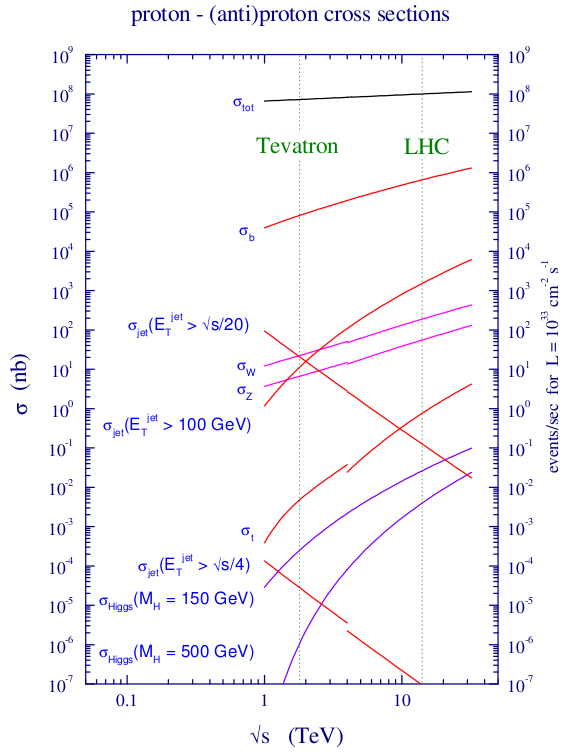
\includegraphics[width=0.8\textwidth]{xsec.png}
  \caption{The production cross sections as a function of centre of mass energy
for several Standard Model and new physic processes.}
  \label{fig:LHCxsec}
\end{figure}

\FigureRef{fig:LHCxsec} shows various cross sections for several physics
processes as a function of the centre of mass energy. The cross section for many
physics processes of interest, such as the Higgs cross section, are several
orders of magnitude below the total inelastic cross section and increase as a
function of centre of mass energy. This motivates the need for a collider with a
very large luminosity as well as a large centre of mass energy.

The LHC is part of a larger accelerator complex as shown in figure
\FigureRef{fig:LHCcomplex}. First Hydrogen gas is ionised to produce a cloud of
protons, which are then accelerated by the LINAC2 linear accelerator to
\unit{50}{\MeV}.

Before being injected in to the Proton Syncrotron (PS) the protons are injected in to
the Proton Syncrotron Booster (PSB) and accelerated to \unit{1.4}{\GeV}. In the
PS the protons are formed in to bunches and the energy is increased to
\unit{25}{\GeV}. The bunches are then accelerated in the Super Proton
Syncrotron (SPS) to \unit{450}{\GeV} and then injected in to the LHC.

%bunches?

\begin{figure}[htb!]
  \centering
  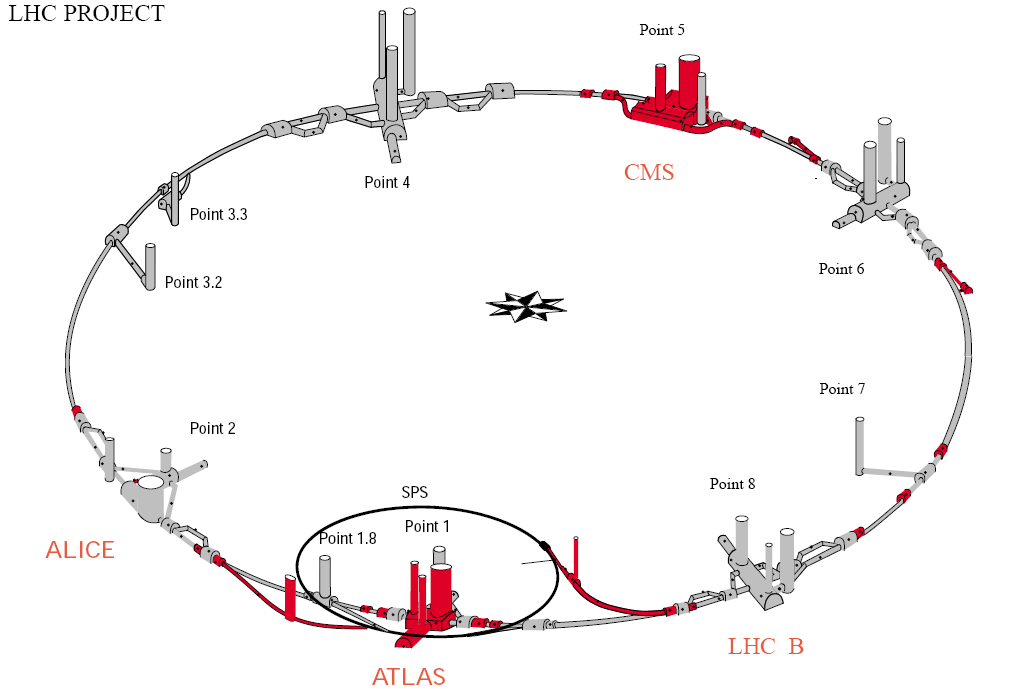
\includegraphics[width=0.8\textwidth]{LHC}
  \caption{The LHC complex.}
  \label{fig:LHCcomplex}
\end{figure}

There are four main detector experiments studying the collisions at the LHC. 
ALICE (A Large Ion Collider Experiment) is designed to study the quark gluon
plasma that will be produced in the heavy ion collisions. 
LHCb (The Large Hadron Collider beauty) experiment is designed to study B-meson
decays to measure CP violation. 
ATLAS (A Toroidal Lhc ApparatuS) and CMS (Compact Muon Solenoid) are general
purpose detectors that are designed 
to search for a wide range of new physics.\cite{lhc}

\subsection{Operational History}
In September 2008 the LHC was commissioned and the first beams were circulated.
Before the first collisions could be delivered an interconnection
between two of the dipole magnets failed when the magnet quenched.
This led to a large ammount to helium evaporating which in turn led to
considerable damage to the machine.

Due to this incident it was decided that the LHC should be run at a lower centre
of mass energy of \unit{7}{\TeV} until the quench protection system could be
upgraded.

The LHC was repaired by the end of 2009 and the first collisions at a record
energy of \unit{2.36}{\TeV} were delivered in November. 
From March to November 2010 The LHC operated at \unit{7}{\TeV} delivering
\unit{46.4}{\invpb} of proton-proton collisions as shown in
\FigureRef{fig:LHC2010}.

\begin{figure}[htb!]
  \centering
  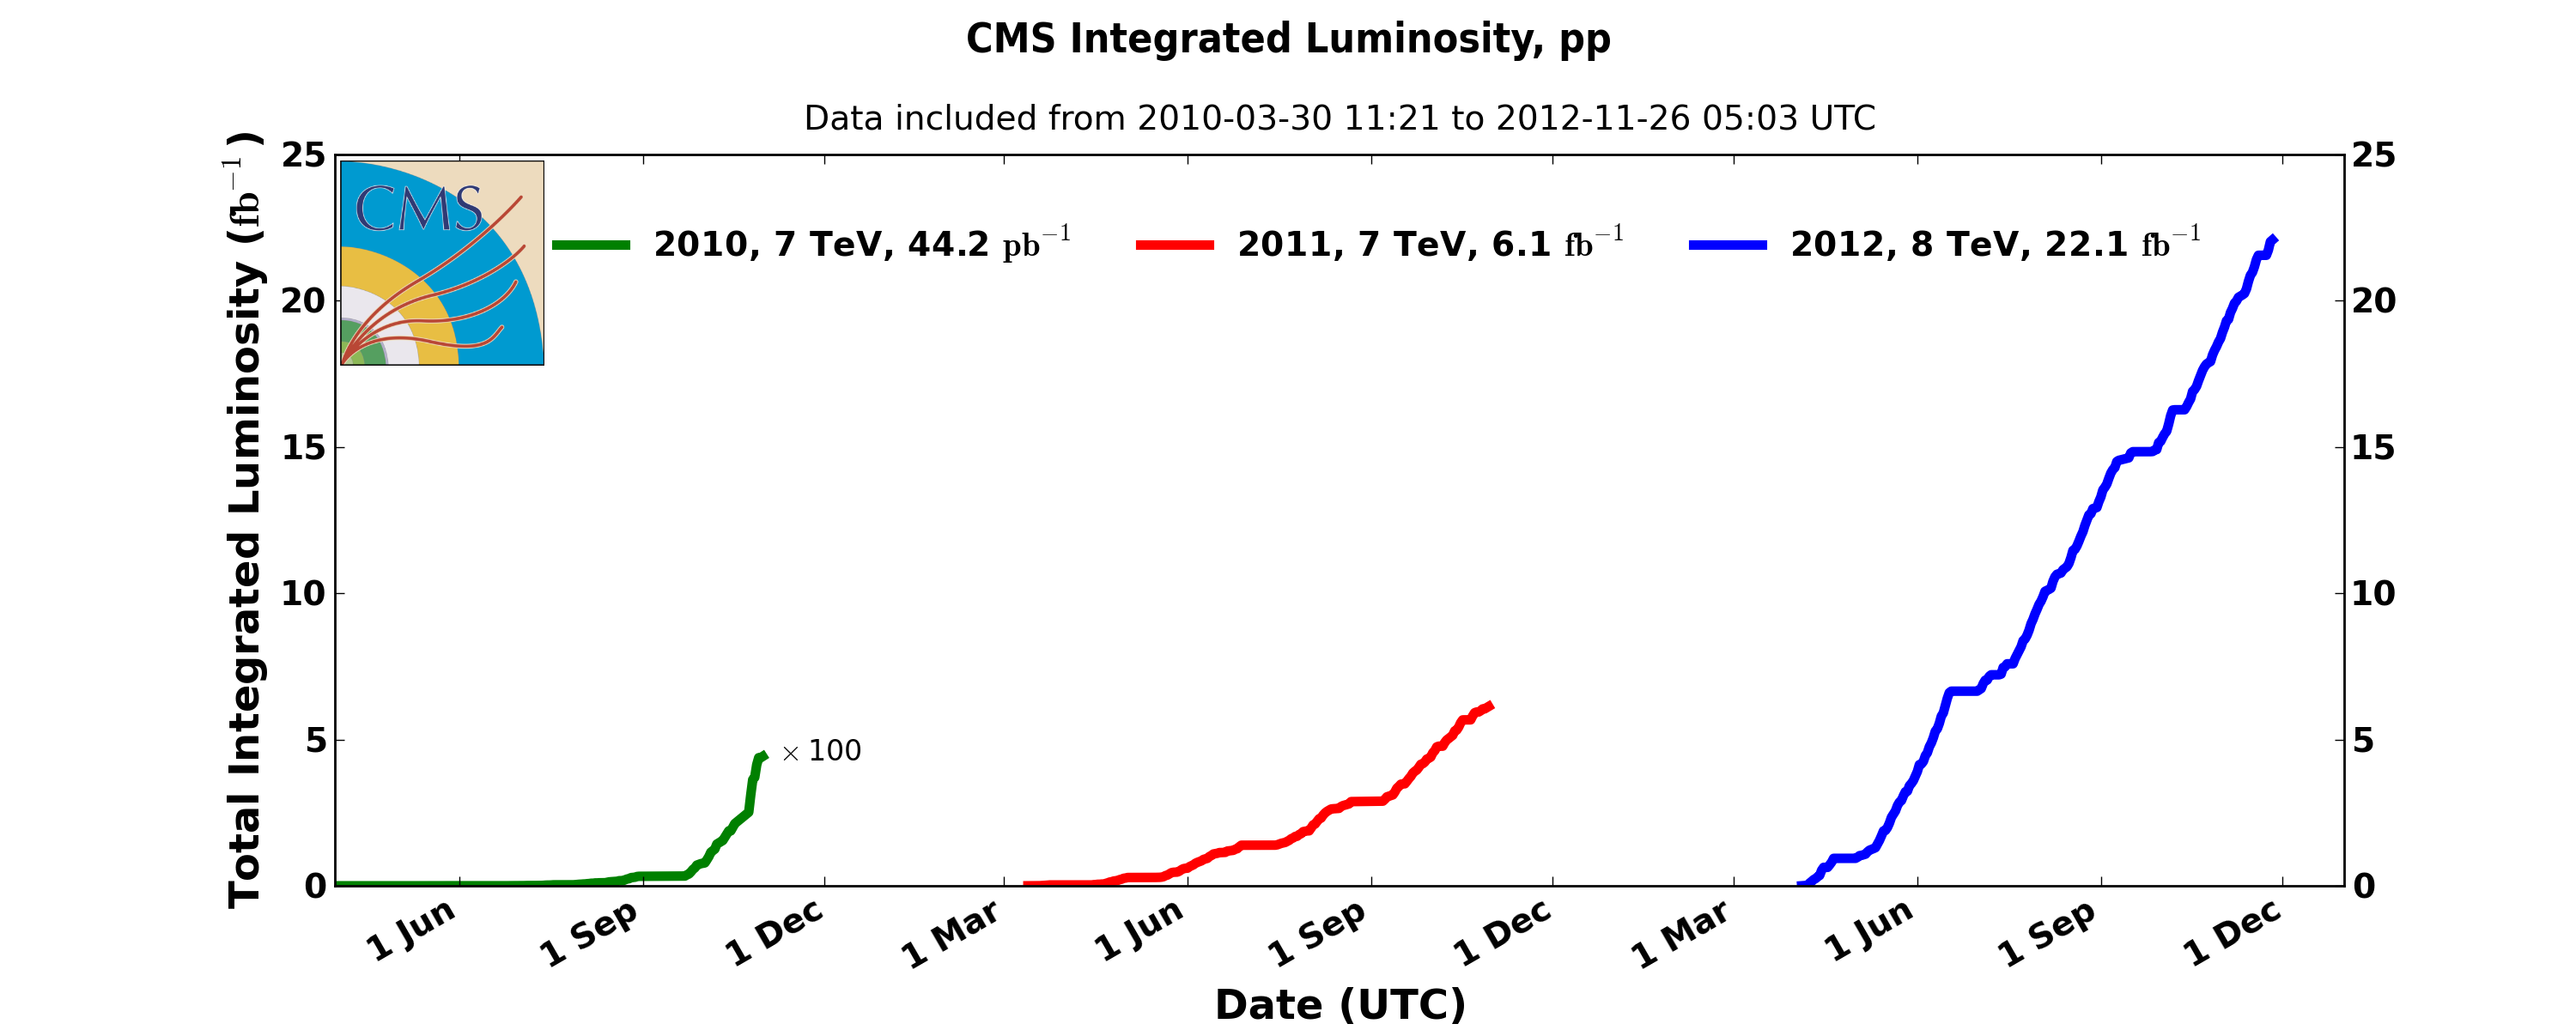
\includegraphics[width=\textwidth]{int_lumi_cumulative_pp_1.png}
  \caption{The luminosity delivered by LHC in 2010}
  \label{fig:LHC2010}
\end{figure}

In November and October 2010 the LHC produced lead ion collisions at
\unit{2.36}{\TeV}.

The target for running in 2011 was to deliver \unit{1}{\invfb} of data. This was
achieved by June. The target was changed to \unit{5}{\invfb} of data by the end
of the yeah which was achieved by October.

\subsection{Physics Goals}
% design goals

\subsection{Experimental Challenge}
%challenges


\section{CMS detector}
CMS (Compact Muon Solenoid)\cite{cms} is one of the two general purpose
detectors designed to study LHC collisions. 

An overview of the detector is shown in figure 
\begin{figure}[htb!]
  \centering
  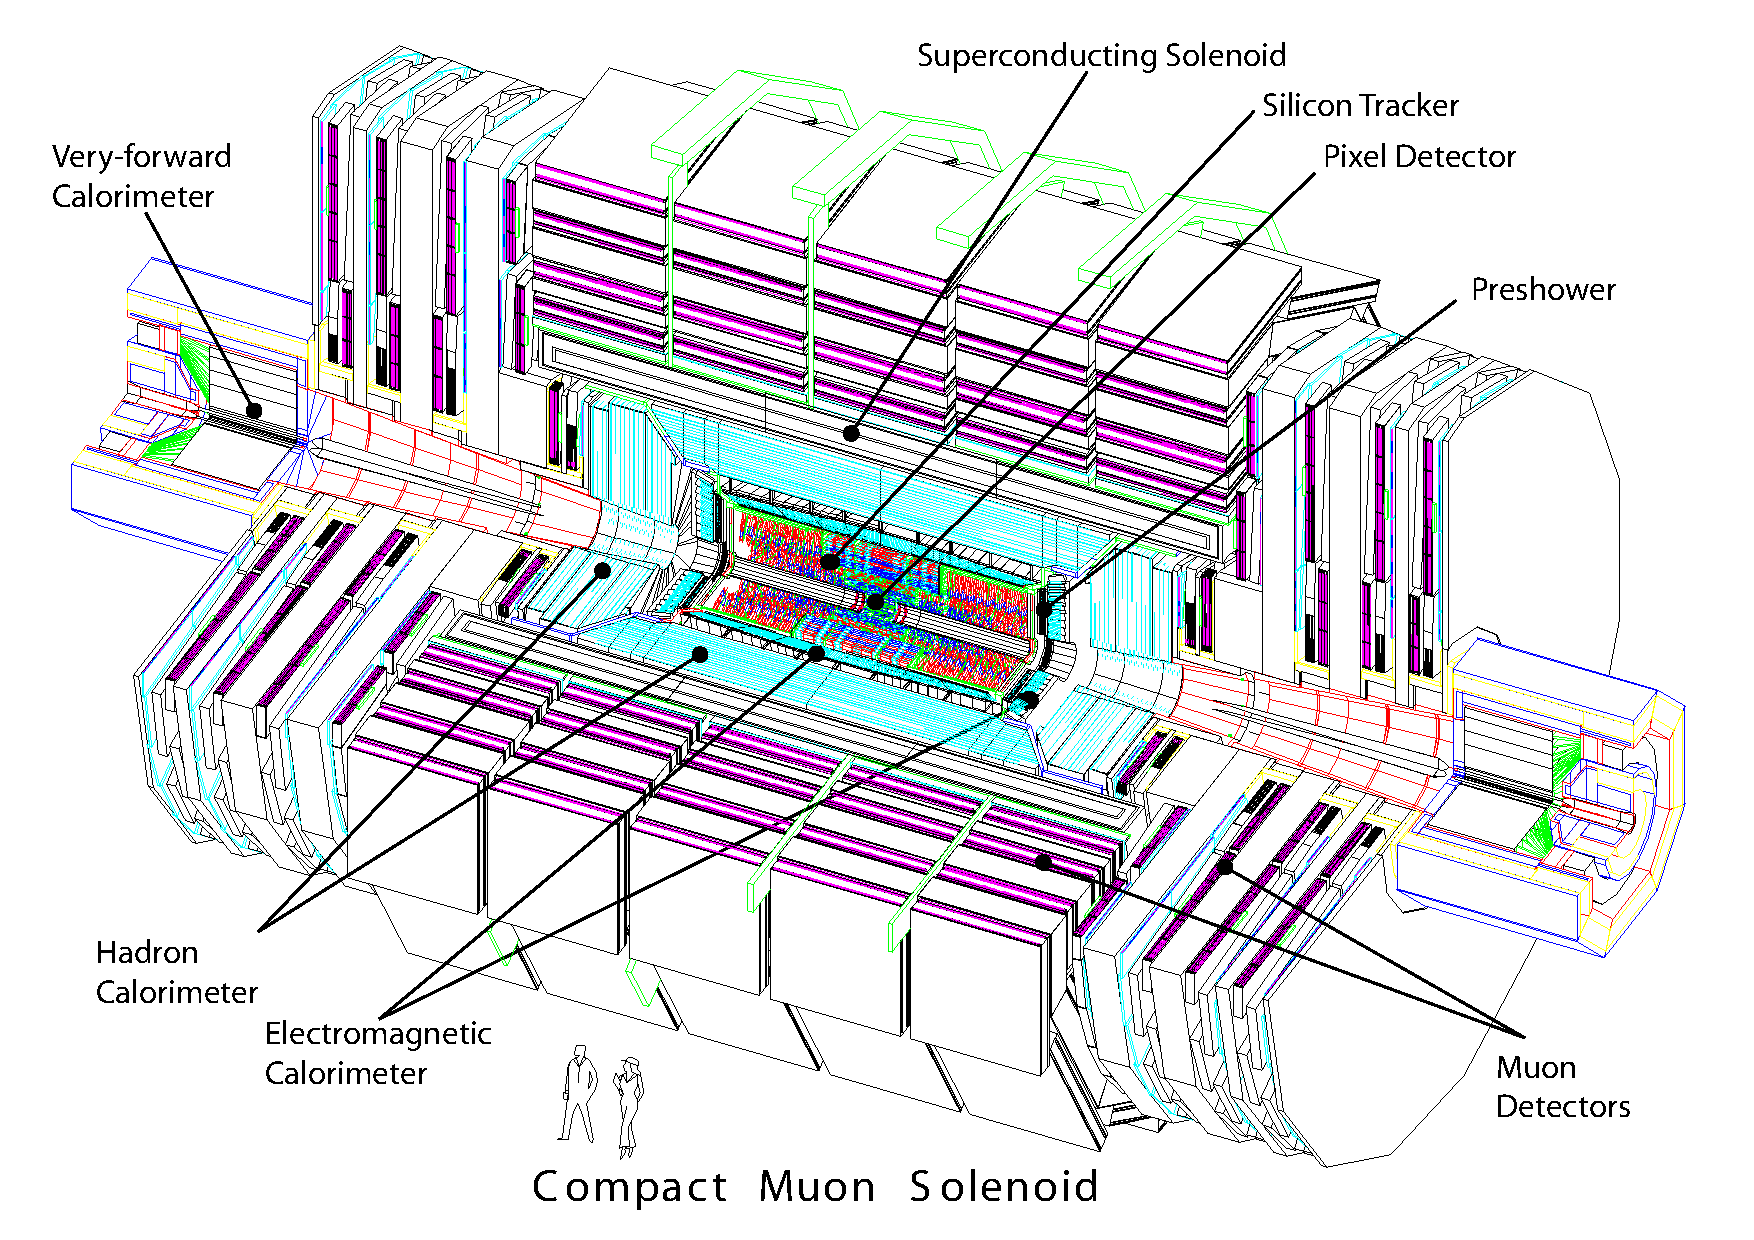
\includegraphics[width=0.8\textwidth]{cms}
  \caption{Diagram of the CMS detector. From \cite{cms}}
  \label{fig:CMSnc}
\end{figure}

Starting at the interaction point at the centre of the detector and moving
radially outwards there is the pixel tracker, silicon tracker, lead-tungstate
ECAL, the sampling brass-plate HCAL, the \unit{4}{\tesla} superconducting
solenoid magnet, an outer HCAL and four muon chambers.

\subsection{Magnet}
A large superconducting solenoid that produces a magnetic field of
\unit{4}{\tesla} provides the basis for the design of the CMS detector, and is
the main structural support for the detector componets in the barrel region.

The superconducting magnet in CMS is designed to produce a \unit{4}{\tesla}
field in a bore of 
\unit{6}{\meter} diameter and \unit{12.5}{\meter} length.
While operating at full current the magnet stores \unit{2.6}{\giga\joule} of 
energy.
A large magnetic field is needed to give CMS a large bending power and the
ability to precisely measure the momentum of high-energy charged particles.
The solenoid bore is large enough that the tracking detectors and the
calorimetry can fit inside it.\cite{cms}

The magnetic flux is returned through a \unit{1.8}{\meter} thick saturated iron
yoke which is interleaved with the muon detector.

\subsection{Tracking}
The inner tracker is designed to accurately and efficiently measure the
trajectories of charged particles produced in collisions at the centre of CMS.
The tracker is also required to be able to reconstruct secondary vertices
caused by the decay of a long lived particle.
At the design luminosity of the LHC it is expected that every 25 ns an average
of 1000 particles will traverse the 
inner detector therefore it is required that the inner tracker has a high
granularity and a fast response while 
resilient to radiation damage. 

Formed of silicon pixel detectors in the inner most layers where the particle
flux is the highest.
Outside of that the tracking detector also utilises 10 layers of silicon
micro-strip detectors.

The total active area of silicon in the CMS tracker is over
\unit{200}{\meter\squared}.\cite{cms}

\subsubsection{Pixel Tracker}
The inner most part of the CMS tracker uses hybrid silicon pixel detectors arranged in
the barrel section in three layers, at radii of  44 73 and \unit{102}{\mm}, and in
each endcap region two disks at a $|Z|=340$ and \unit{465}{\mm}.

Each pixel has a surface area of \unit{100x150}{\micron} with an
average particle density of $\mathcal{O}(10^{-4})$ per crossing.

The pixel tracker has $\approx 45\times 10^{6}$ readout channels which are used
to seed the track reconstruction.

\subsubsection{Strip Tracker}
Further from the interaction point the particle flux is much reduced allowing
for the use of silicon strip detectors. 

The barrel tracker comprises two parts, the inner (TIB) and outer (TOB)
trackers. The TIB and TOB are formed of 4 and 6 layers respectivly.

The endcaps are separated in two the Tracker End Cap (TEC) and the Tracker Inner
Disks (TID). The TEC is split in to nine disks and covers the region
$\unit{1200}{\mm} < |Z| < \unit{2800}{\mm}$. The TID comprises three rings
and fills the gap between the TEC and the TIB.

The silicon strip detector consists of under 15400 modules with approximately 10
million readout channels.

\subsection{Electromagnetic Calorimetry}
The electromagnetic calorimeter (ECAL) is 
designed to measure the energy of
particles with a high resolution and granularity.

It is a hermetic, homogenous calorimeter comprising 61200 individual lead
tungstate ($PbWO_{4}$) scintillation crystals in the barrel region
($|\eta|<1.479$) closed by 7324 crystals in each of the two endcap parts
($1.479<|\eta|<3.0$).

Lead tungstate crystals are ideally suited for this since the scintillation
decay time is similar to the LHC bunch crossing time, 
with \unit{80}{\%} of light being produced within \unit{25}{\ns}.
They also have a short radiation lengths ($X_0=\unit{0.89}{\cm}$) 
and Moliere length (\unit{2.2}{\cm}) as well nas being radiation hard
(up to \unit{10}{\mrad}).

A disadvantage to using lead tungstate is that the light output of the crystals
is relatively low and changes with temperature. This is overcome by maintaining
a stable temperature (within \unit{0.1}{\degreecelsius}) and the use of
photodetectors with intrinsic gain.

Silicon avalanche photodiodes (APDs) are used to detect the scintillation light
in the barrel and vacuum phototriodes (VPTs) are used in the endcap parts.

The barrel section of the ECAL (EB) surrounds the inner tracker. It is comprised
of 36 identical supermodules that each cover a half of the length of the barrel
($0<|\eta|<1.479$) and \unit{20}{\degree} in phi. Each supermodule contains
1700 crystals arranged in a $\phi - \eta$ grid with each crystal mounted in a
``semi-projective'' geometry, with each crystal set \unit{3}{\degree} off the
nominal interaction vertex. Each crystal has a cross-section of
\unit{$22 \times 22$}{\mm\squared} and a length of
\unit{230}{\mm}(\unit{25.8}{X_0}).

The endcaps (EE) are formed of two ``Dees'', semi-circular aluminium plates
which support the supercrystals, 5x5 arrays of crystals. The crystals are
mounted off the nominal interaction vertex by a small angle. Unlike the barrel
the crysals are arranged in an x-y grid.
Installed in front of the endcap ECAL is a preshower system which allows for
the rejection of \Ppizero .\cite{cms}

\begin{figure}[htb!]
  \centering
  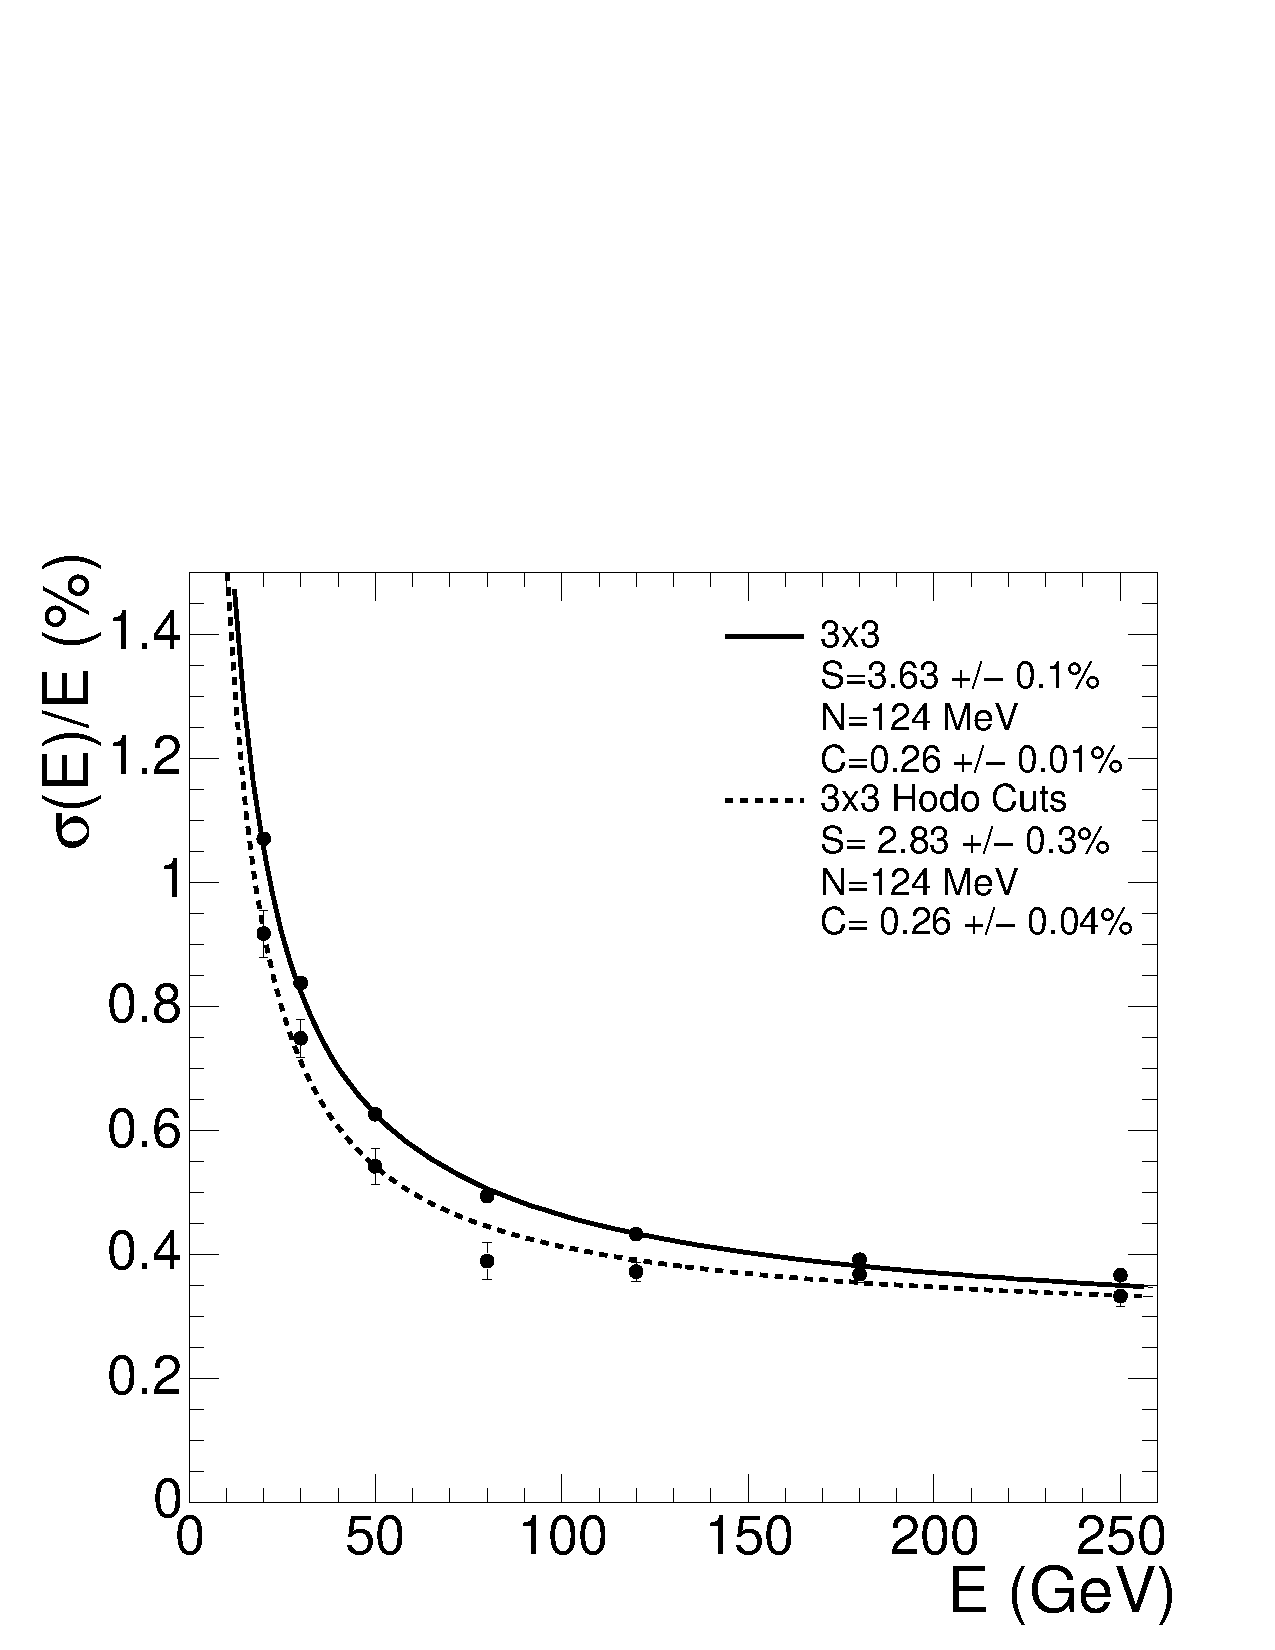
\includegraphics[width=0.6\textwidth]{ecal_performance}
  \caption{Energy resolution $\frac{\sigma}{E}$ of ECAL as a function of
  \label{fig:ECAL}
electron energy $E$. From \cite{cms}.}
\end{figure}

The ECAL energy resolution is shown in figure \ref{fig:ECAL} for test beam
electrons at several energies ($E$) and is fitted with the function
\begin{equation}
\left(\frac{\sigma}{E}\right)^{2} = \left(\frac{S}{\sqrt{E}}\right)^{2} +
\left(\frac{N}{E}\right)^{2} + C^{2}
\end{equation}
where S is the stochastic, N is the noise and C is the constant terms. The
stochastic term is due to the statistical fluctuations in the particles
produced in the electromagnetic shower. The noise term is due to electronic
noise and pile-up and is independent of energy. The constant term is due to
errors that are independant of energy, such as non-uniform signal generation
and calibration errors.\cite{cms}

% \subsubsection{ECAL Spikes!?}


% \subsubsection{ECAL Endcap Misalignment!?}
% It was found in early data taking that the ECAL endcaps are misaligned with
% respect to the tracker. This causes problems when reconstructing electrons
% since the difference between the track position and ECAL energy deposit is a
% variable that is cut on in the electron candidate selection. As a quick fix
% to this problem, an 

\subsection{Hadronic Calorimetry}

The Hadronic Calorimeter (HCAL) is designed to measure the energy of
hadron jets and the missing transverse energy (\met) which are important
signatures in many New Physics searches.

The HCAL s a brass/scintillator sampling hadron calorimeter that covers the
region up to $|\eta|<3.0$.
The scintillation light is channelled by wavelength shifting fibres, that are
embedded in the scintillation tiles, to hybrid photodiodes that can operate in
the high magnetic field. \cite{cms}

The HCAL comprises four components: the hadron barrel (HB), hadron outer (HO),
hadron endcap (HE) and the hadron forward (HF).

The hadron barrel covers the region ($|\eta| < 1.4$) and is positioned between
the ECAL and inside of the solenoid magnet coil
($\unit{1.77}{\meter}<R<\unit{2.95}{\meter}$).
This constrains the design of the HCAL and limits the total amount of material
to absorb the hadronic shower. 
To overcome this limitation the outer hadronic calorimeter is
placed outside the solenoid to complement the HCAL barrel and increases the
effective thickness of the hadron calorimetry to over 10 interaction lengths.

The hadron barrel covers the region $1.3 < |\eta| < 3.0$.

In the forward region $|\eta| > 3$ energy measurements are made with an
iron/quartz-fibre forward hadronic calorimeter where the Cherenkov light is
detected by photodetectors. The calorimeter needs to be radation hards as in the
forward range the particle flux is very large.

\begin{figure}[htb!]
  \centering
  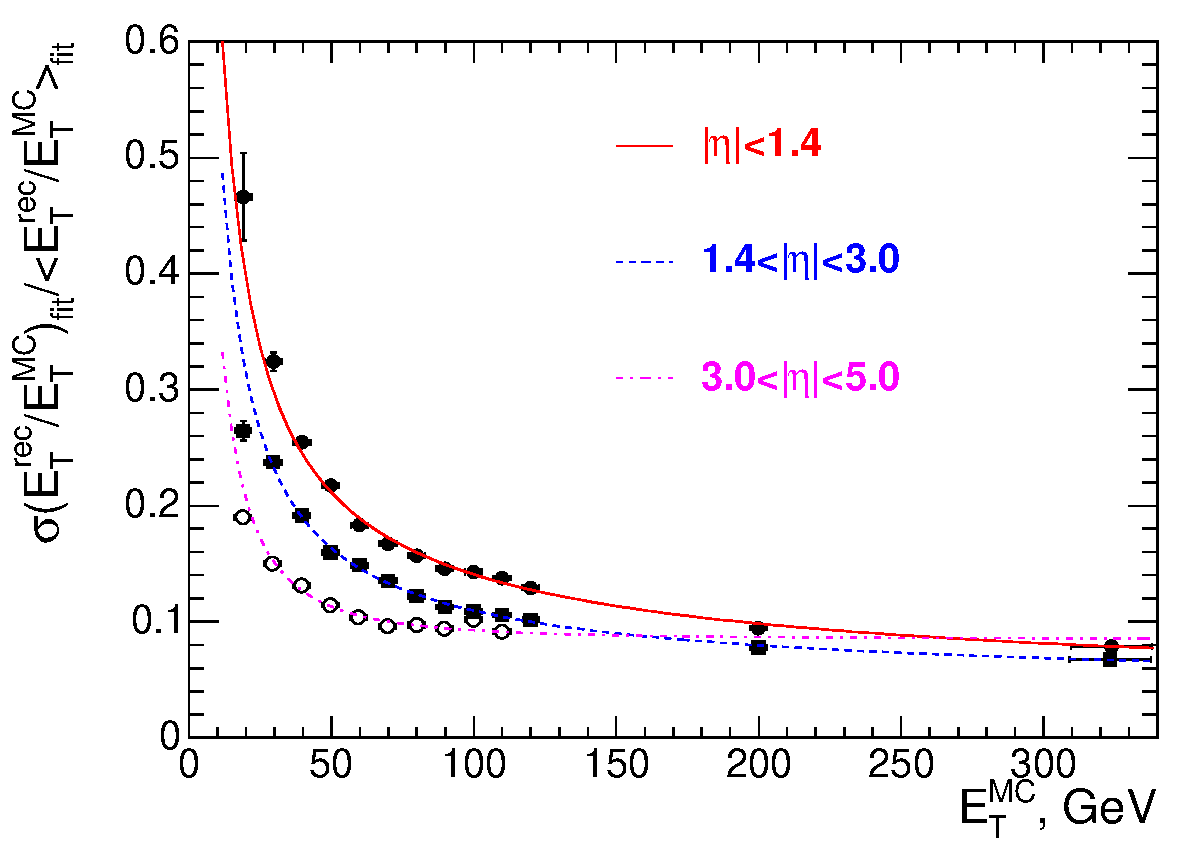
\includegraphics[width=0.8\textwidth]{hcal_performance}
  \caption{Energy resolution $\frac{\sigma}{E}$ of HCAL as a function of jet
  \label{fig:HCAL}
transverse energy for barrel jets ($|\eta| < 1.4$), endcap jets ($1.4<|\eta| <
3$) and forward jets $3<|\eta| < 5$). From \cite{cms}.}
\end{figure}


\subsection{Muon System}
The muon system lies outside of the CMS solenoid and the outer HCAL detectors,
it is designed to have three functions; to identify muons, measure the momentum
of muons and trigger on muons; to perform these functions the muon system
consists of several different types of detectors.

\begin{figure}[ht]
  \centering
  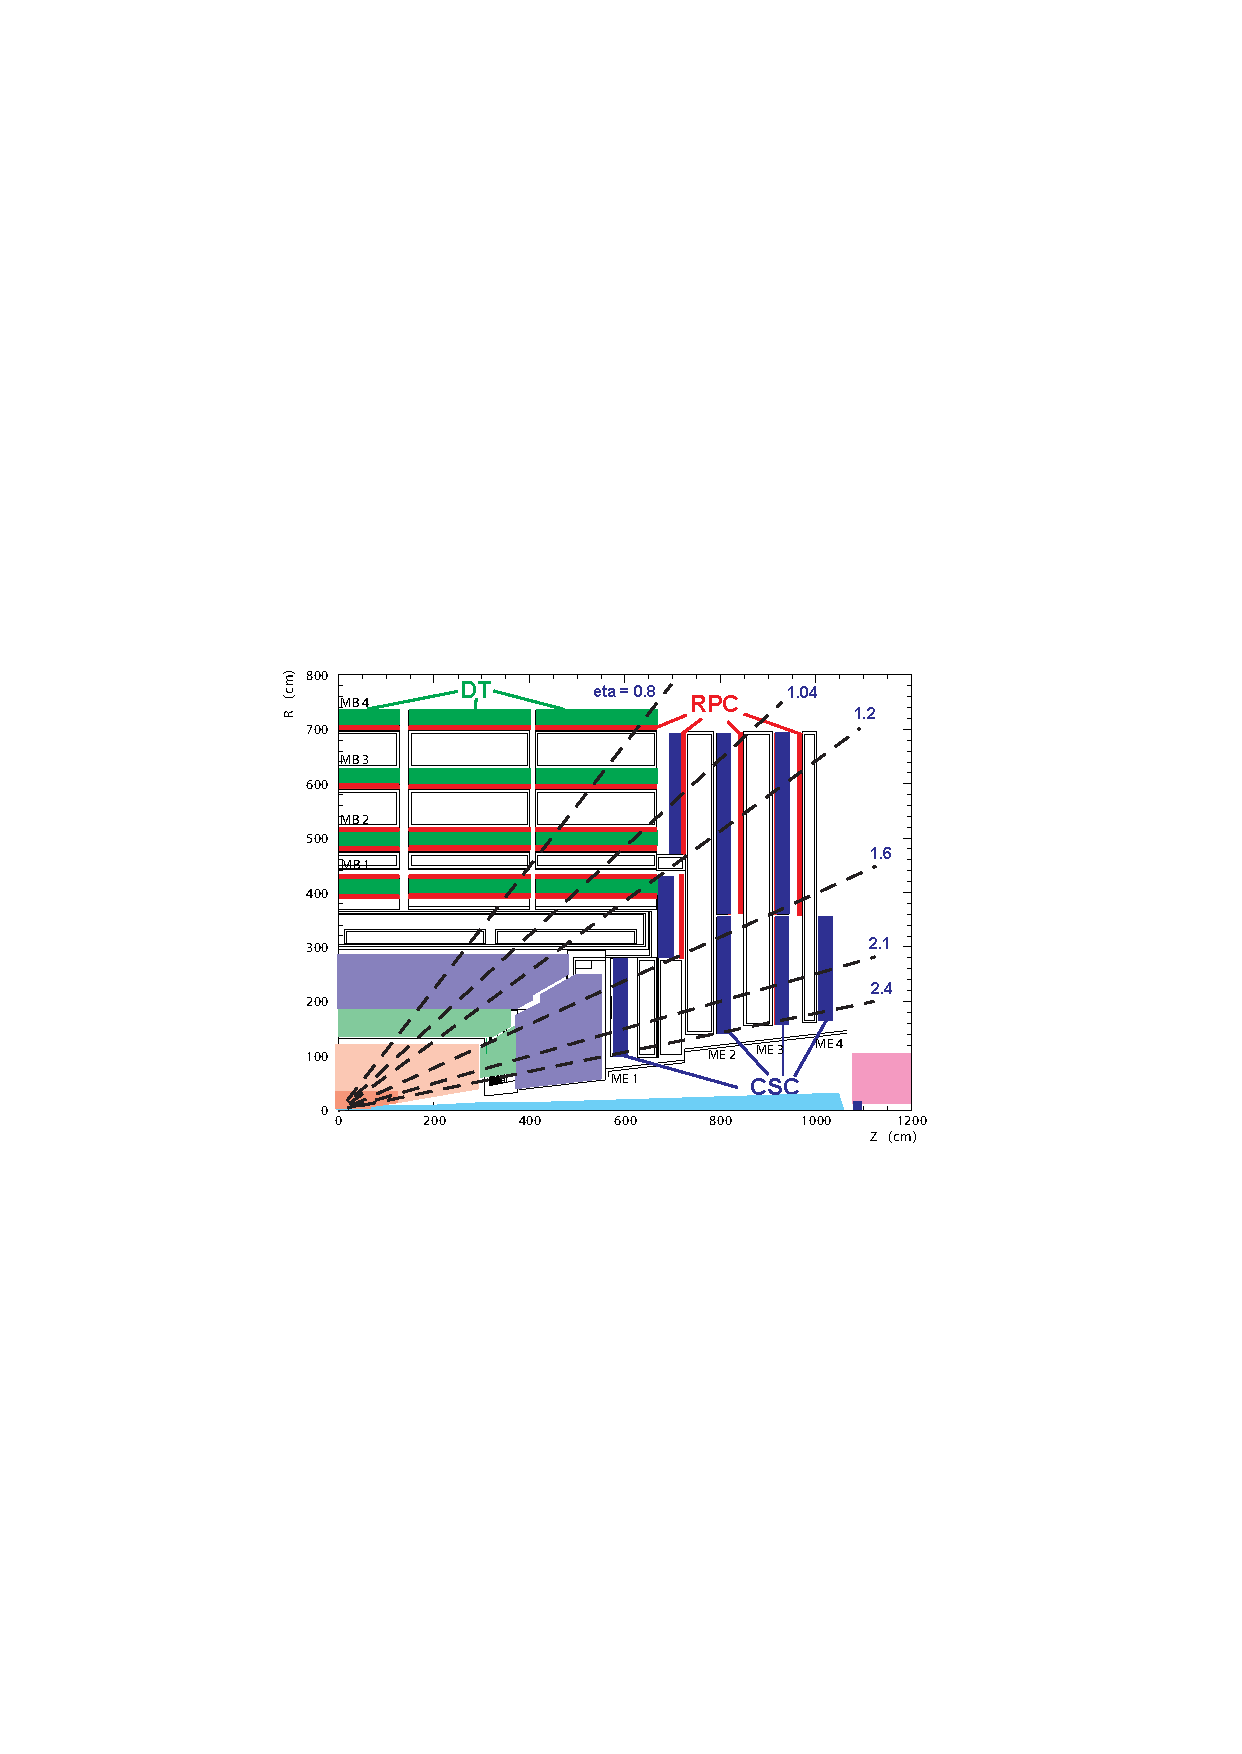
\includegraphics[width=0.8\textwidth]{muon_system}
  \caption{Muon system}
  \label{fig:muon_system}
\end{figure}

\subsubsection{Drift Tubes}
In the barrel region ($|\eta| < 1.2$) aluminium drift tubes (DT) are used
arranged in four stations interspersed along the layers of the flux return
plates. 
Each station contains 12 layers, eight to measure the coordinate in the
$r-\phi$ plane and four to measure the $z$ direction (except the fourth station
which only measures the $r-\phi$ plane). 

\subsubsection{Cathode Strip Chambers}
In the endcaps ($0.9<|\eta|<2.4$) cathode strip chambers (CSC) are used. The
CSCs are arranged in to four stations in each endcap arranged so they are
perpendicular to the beam line, and are placed between the flux return plates.
The cathode strips of each chamber run radially away from the beam line where
as the anode wires run perpendicular to the strips; both are read out which
gives information on both the $r-\phi$ plane (from the cathode) and the $\eta$
direction (from the anode). \cite{cms}

\subsubsection{Resistive Plate Chambers}
In addition to DT chambers and CSCs a complimentary trigger system is also used
consisting of resistive plate chambers (RPC) in the endcap and barrel regions.
The RPCs are able to provide a fast and independent trigger over a large range
($|\eta| < 1.6$). In the barrel region, 6 layers of RPCs are used, 2 in each of
the first 2 muon stations and 1 in each of the last 2 stations. In the endcap a
layer of RPCs in each of the first 3 stations.

An optical alignment system, that uses lasers and LEDs, measures the positions
of each muon station with respect to each other and the CMS inner tracker to
ensure an accurate and high resolution measurement of the muon
momentum.\cite{cms}

The performance of the muon system and inner tracker is shown in figure
\ref{fig:MS}.

\begin{figure}[htb!]
  \centering
  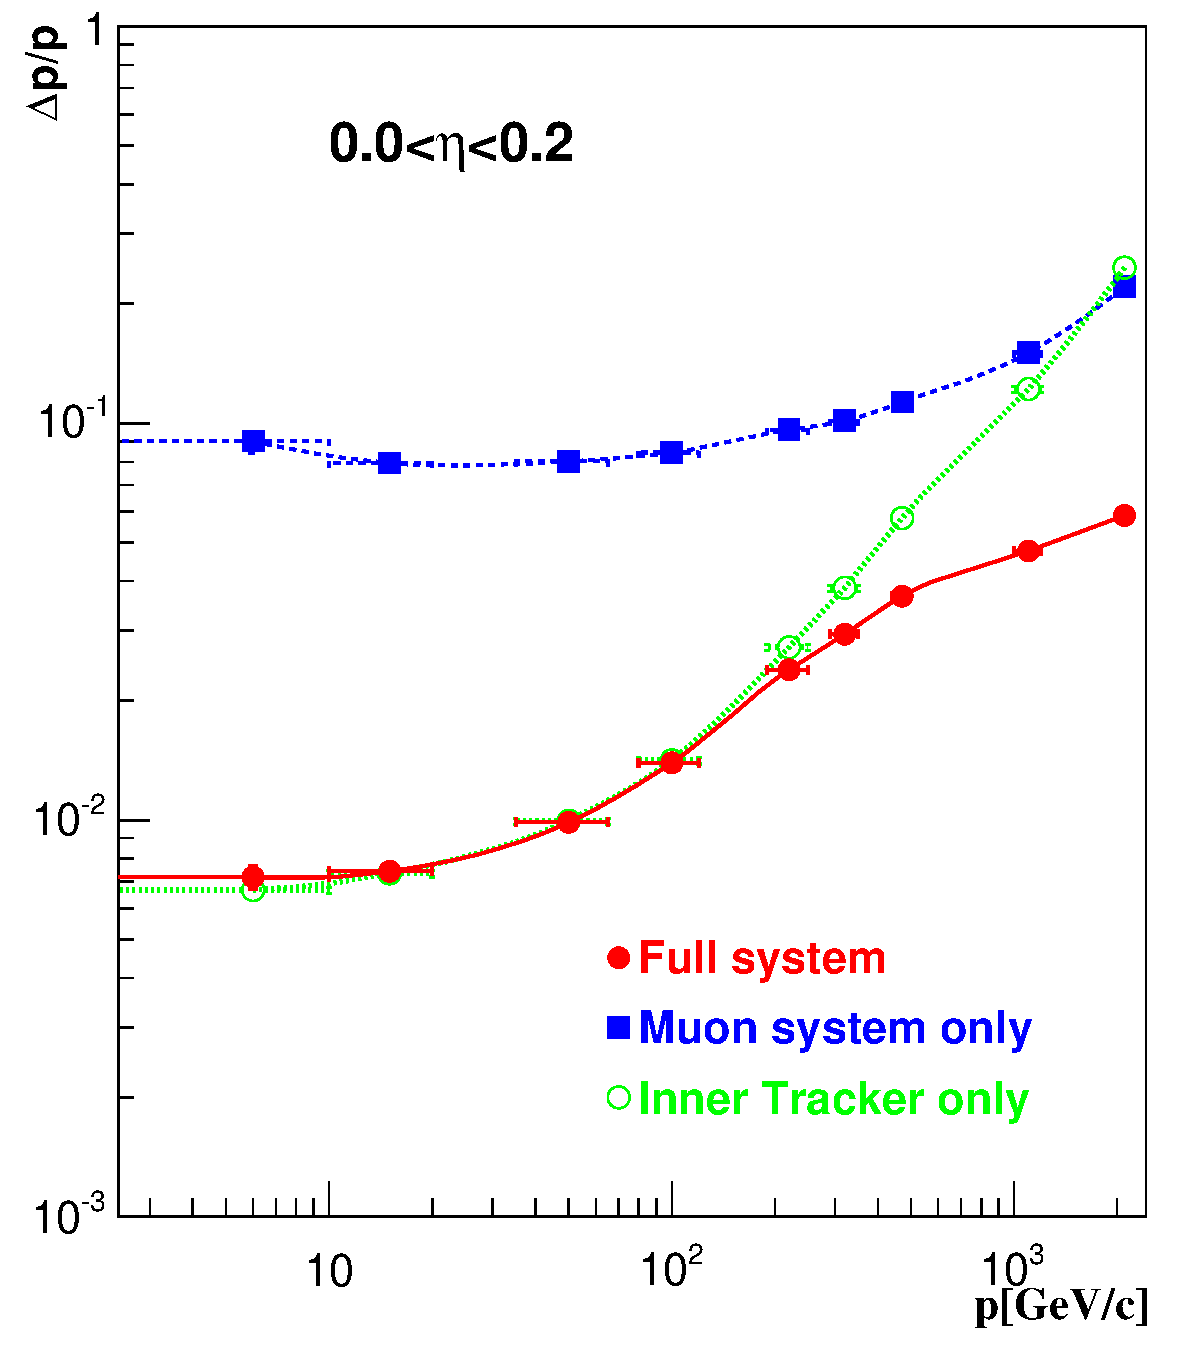
\includegraphics[width=0.45\textwidth]{muon_barrel}
  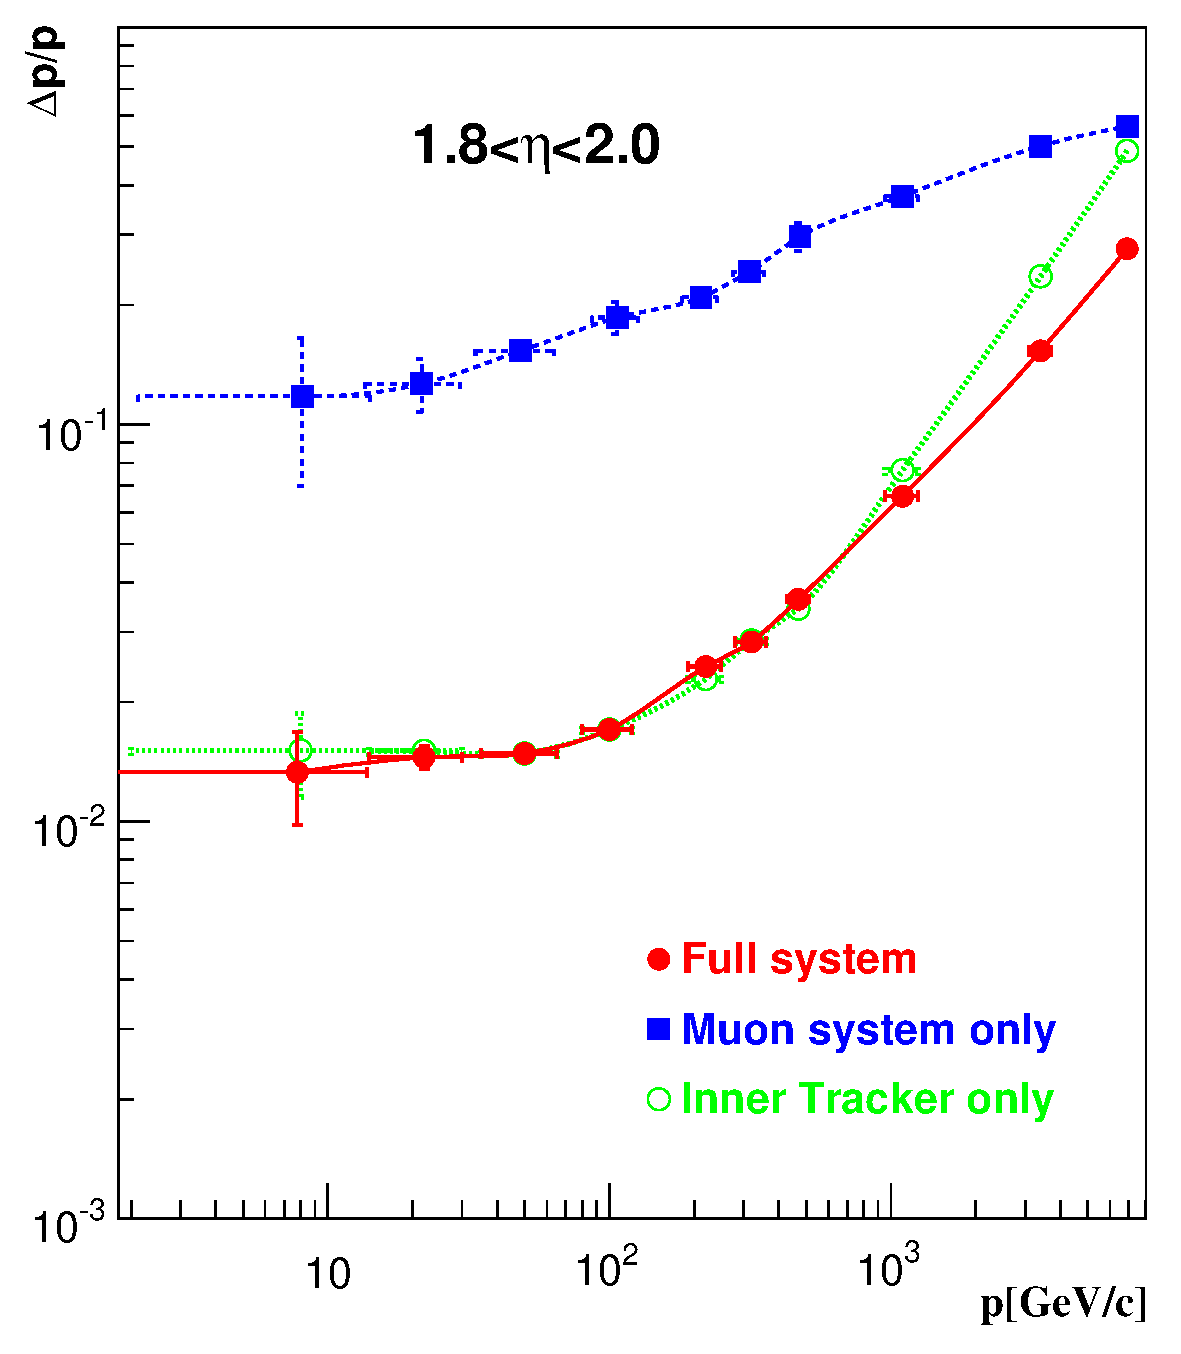
\includegraphics[width=0.45\textwidth]{muon_endcap}
  \caption{Muon transverse momentum resolution as a function of the
  \label{fig:MS}
transverse-momentum using only the muon system, only the tracker and both, for
left, barrel muons ($|\eta| < 0.8$) and right, endcap muons ($1.2<|\eta| <
2.4$). From \cite{cms}.}
\end{figure}


\subsection{Trigger and Data Acquisition}
At design luminosity, the high bunch crossing frequency of the LHC means that
CMS will observe a collision containing an average of 20 superimposed inelastic
events every \unit{25}{\nano\second}, a rate of $10^{9}$ interactions per
second.
A zero suppresed event output from CMS is about \unit{2}{MB} so the total data
output rate from CMS is \unit{$\approx 80$}{TB \per \second},  however data from
only about $10^{2}$ crossings can be written to the tape storage. 

The vast majority of events will contain only inelastic collisions and not be of
interest from a physics perspective and can be discarded.  
It is the job of the trigger to reduce the rate of events
by a factor of $10^6$ by rejecting the uninteresting events while keeping as
many interesting events as possible.

An overview of the DAQ and trigger is shown in figure \ref{fig:CMSDAQ}.

\begin{figure}[htb!]
  \centering
  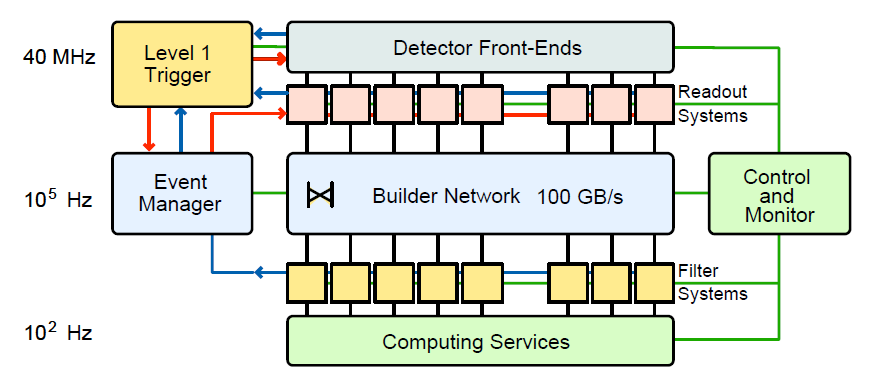
\includegraphics[width=0.6\textwidth]{CMSDAQ}
  \caption{Overview of the architecture of the CMS DAQ and trigger. From
  \label{fig:CMSDAQ}
\cite{cms}.}
\end{figure}

The trigger is separated in to two parts the Level-1 (L1) trigger and the High
Level Trigger (HLT).\cite{cms}

\subsubsection{Level-1 Trigger}




The Level-1 trigger is designed to reduce the event rate from the bunch
crossing frequency of \unit{40}{\mega\hertz} to a maximum output rate of
\unit{100}{\kilo\hertz}.
This is achieved with custom-designed fast programmable electronics that takes
as input coarsely segmented data from the calorimeters and muon systems and
places the high resolution data in pipelined memories.



\subsubsection{High-Level Triggers}
The high-level trigger is a software system which runs on a server farm with
over one thousand commercial multi-core processors with access to the complete
event data allowing it to make more complex calculations. After the L1 trigger
and HLT the rate is reduced by a factor of $1 \eexp 6$ and is output to mass
storage.\cite{cms}

